%%%%%%%%%%%%%%%%%%%%%%%%%%%%%%%%%%%%%%%%%%%%%%%%%%%
%% LaTeX book template                           %%
%% Author:  Amber Jain (http://amberj.devio.us/) %%
%% License: ISC license                          %%
%%%%%%%%%%%%%%%%%%%%%%%%%%%%%%%%%%%%%%%%%%%%%%%%%%%

\documentclass[a4paper,11pt]{book}
\usepackage[T1]{fontenc}
\usepackage[utf8]{inputenc}
\usepackage{lmodern}
%%%%%%%%%%%%%%%%%%%%%%%%%%%%%%%%%%%%%%%%%%%%%%%%%%%%%%%%%
% Source: http://en.wikibooks.org/wiki/LaTeX/Hyperlinks %
%%%%%%%%%%%%%%%%%%%%%%%%%%%%%%%%%%%%%%%%%%%%%%%%%%%%%%%%%
\usepackage{hyperref}
\usepackage{graphicx}
\usepackage[english]{babel}
\usepackage[a4paper,top=2cm,bottom=2cm,left=2cm,right=2cm]{geometry}
\usepackage{lscape}
\usepackage{caption}
\usepackage{amsmath}
\usepackage{listingsutf8}
\usepackage{float}
\usepackage{amsmath}
\usepackage{subfig}

\usepackage{wrapfig}
\usepackage{rotating}
\usepackage{epstopdf}

\usepackage[ruled]{algorithm2e}
\lstset{% general command to set parameter(s)
	basicstyle=\small, % print whole listing small
	numbers=left,
	keywordstyle=\color{black}\bfseries,
	% underlined bold black keywords
	identifierstyle=, % nothing happens
	stringstyle=\ttfamily} % typewriter type for strings

\lstset{language=Java} 
\captionsetup{tableposition=top,figureposition=bottom,font=small}
%%%%%%%%%%%%%%%%%%%%%%%%%%%%%%%%%%%%%%%%%%%%%%%%%%%%%%%%%%%%%%%%%%%%%%%%%%%%%%%%
% 'dedication' environment: To add a dedication paragraph at the start of book %
% Source: http://www.tug.org/pipermail/texhax/2010-June/015184.html            %
%%%%%%%%%%%%%%%%%%%%%%%%%%%%%%%%%%%%%%%%%%%%%%%%%%%%%%%%%%%%%%%%%%%%%%%%%%%%%%%%
\newenvironment{dedication}
{
   \cleardoublepage
   \thispagestyle{empty}
   \vspace*{\stretch{1}}
   \hfill\begin{minipage}[t]{0.66\textwidth}
   \raggedright
}
{
   \end{minipage}
   \vspace*{\stretch{3}}
   \clearpage
}

%%%%%%%%%%%%%%%%%%%%%%%%%%%%%%%%%%%%%%%%%%%%%%%%
% Chapter quote at the start of chapter        %
% Source: http://tex.stackexchange.com/a/53380 %
%%%%%%%%%%%%%%%%%%%%%%%%%%%%%%%%%%%%%%%%%%%%%%%%
\makeatletter
\renewcommand{\@chapapp}{}% Not necessary...
\newenvironment{chapquote}[2][2em]
  {\setlength{\@tempdima}{#1}%
   \def\chapquote@author{#2}%
   \parshape 1 \@tempdima \dimexpr\textwidth-2\@tempdima\relax%
   \itshape}
  {\par\normalfont\hfill--\ \chapquote@author\hspace*{\@tempdima}\par\bigskip}
\makeatother

%%%%%%%%%%%%%%%%%%%%%%%%%%%%%%%%%%%%%%%%%%%%%%%%%%%
% First page of book which contains 'stuff' like: %
%  - Book title, subtitle                         %
%  - Book author name                             %
%%%%%%%%%%%%%%%%%%%%%%%%%%%%%%%%%%%%%%%%%%%%%%%%%%%

% Book's title and subtitle
\title{
	
\includegraphics[width=0.7\textwidth]{Immagini/UniBg.png}
	\\ \Huge \textbf{Navigazione basata su inseguimento di frecce} \\ \huge \textit{\textbf{Relazione di progetto}} \\ \bigskip \huge Progetto del corso Robotica (principi e progetto)\\ Università degli Studi di Bergamo \\ \huge A.A. 2019/2020}
% Author
\author{\textsc{Calegari Andrea - 1041183}
		\\ \textsc{Paganessi Andrea - 1040464}
		\\ \textsc{Piffari Michele - 1040658}}

\begin{document}
	
	\frontmatter
	\maketitle
	%%%%%%%%%%%%%%%%%%%%%%%%%%%%%%%%%%%%%%%%%%%%%%%%%%%%%%%%%%%%%%%%%%%%%%%%
	% Auto-generated table of contents, list of figures and list of tables %
	%%%%%%%%%%%%%%%%%%%%%%%%%%%%%%%%%%%%%%%%%%%%%%%%%%%%%%%%%%%%%%%%%%%%%%%%
	\tableofcontents
	\listoffigures
	
	
	
	\mainmatter
	\chapter{Stato dell'arte}
	Obbiettivo: andare a implementare sistema di \textit{visual navigation} per la base robotica in figura ~\ref{fig:BaseRobotica}.

\begin{figure}
	\centering
	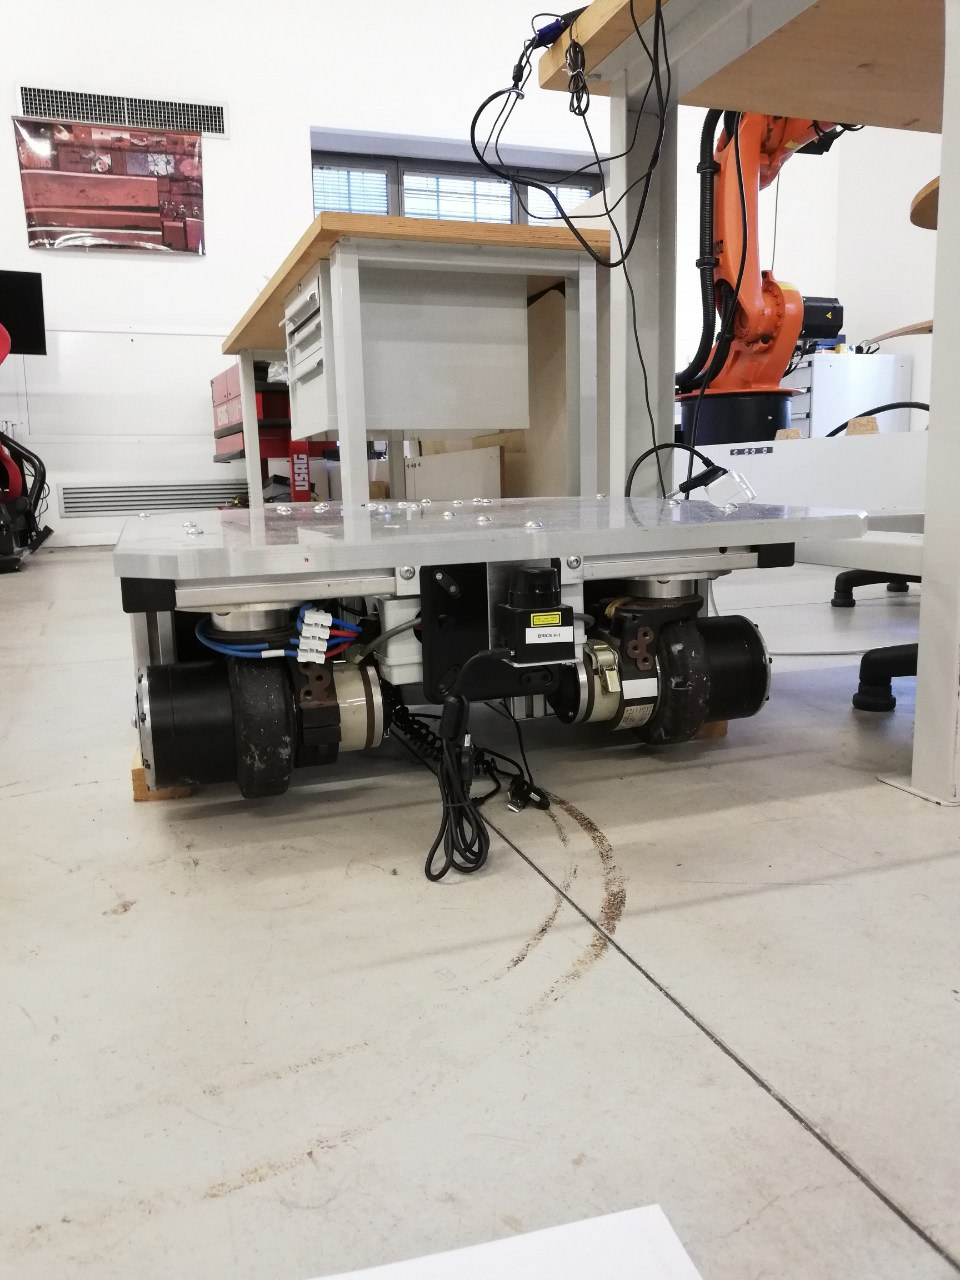
\includegraphics[width=0.5\textwidth]{Immagini/BaseRobotica.jpg}
	\caption{Base robotica addetta alla movimentazione}
	\label{fig:BaseRobotica}
\end{figure}

\begin{figure}
	\centering
	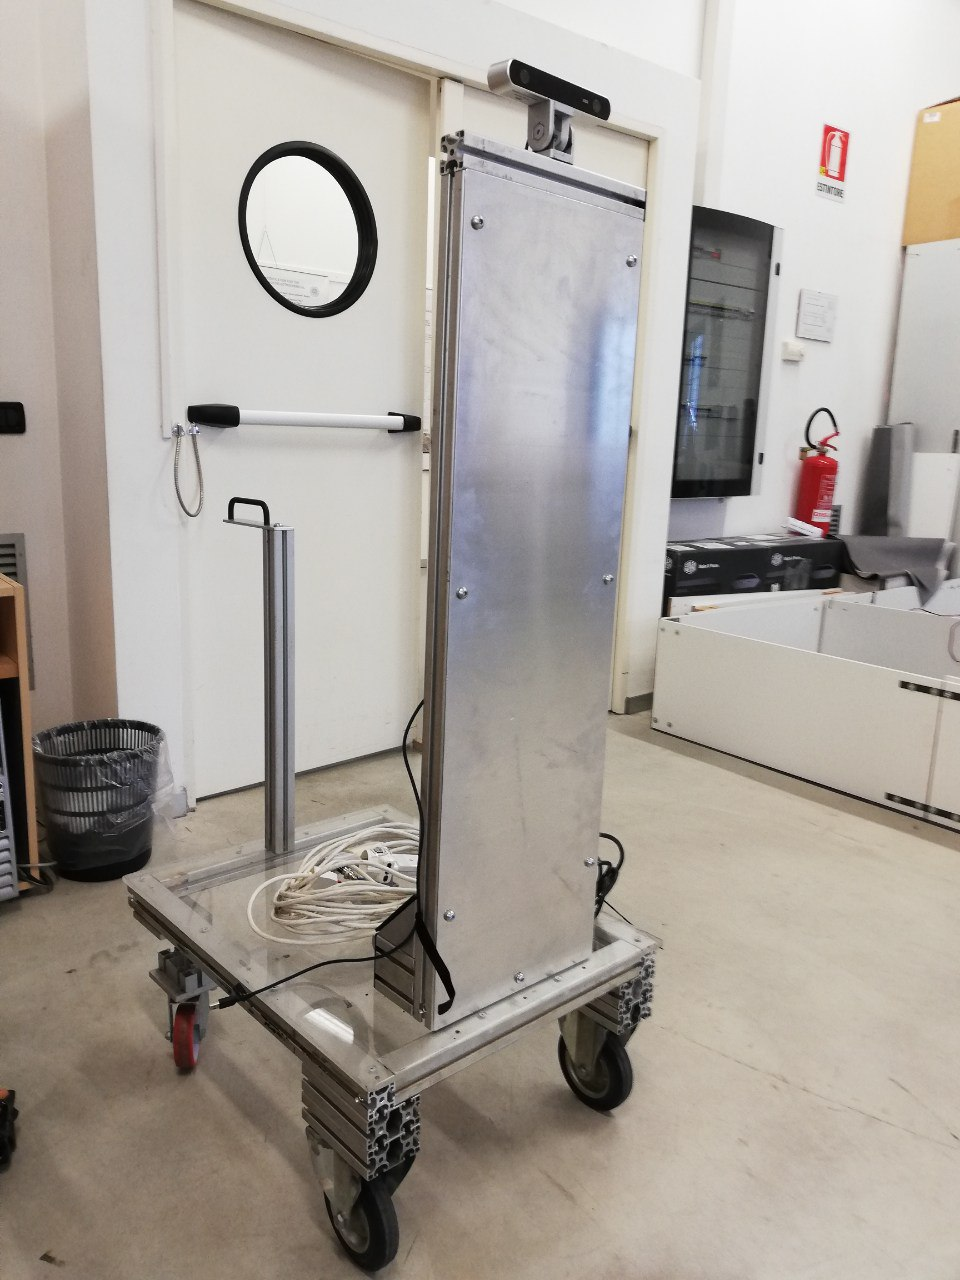
\includegraphics[width=0.5\textwidth]{Immagini/SupportoCamera.jpg}
	\caption{Base verticale sulla quale andare ad inserire la camera}
	\label{fig:SupportoRialzato}
\end{figure}

\section{SAL - Stato avanzamento lavori}
\begin{itemize}
	\item Analizzato codice Out-Of-Box del progetto dello scorso anno
	\begin{itemize}
		\item Il codice preso non aveva main: creato
		\item Compresa struttura pub/sub
		\item Analizzati topic/nodes pubblicati
	\end{itemize}
	\item Cambio camera. Perchè? Prestazioni scarse al variare della luce
	\item Nuova camera --> ueye cam
	\item Fatta funzionare nuova camera
	\begin{itemize}
		\item Demo (programma già fornito con la camera)
		\item Ros --> utilizzato file debug-launch (inserire caratteristiche che la camera fornisce quando parte lo script).
	\end{itemize}
	\item Scelta la posizione della camera: verticale inclinata e non orizzontale
	\item Progetto A.A. utilizza formule vecchie
	\item Problema CPU consuming (problema intrinseco della camera)
	\item Memory problem --> risolto con \textit{free}
	\item Doppie maschere: frecce di due colori
	\item Aggiunte queste features:
	\begin{itemize}
		\item Gaussian blur
		\item Brightness
		\item Erosion - Dilatation
	\end{itemize}
	\item Fatta erosione solo sulle frecce vicine (quelle nella metà inferiore del frame), mentre invece, le frecce nella metà superiore non vengono erose ma solo dilatate.
	\item Problema inizializzazione che mostrava rettangoli bianchi su alcune immagini intermedie nelle maschere
	\item Aggiunta distanza tra centri con tracciamente linea
	\item Prendiamo la freccia più vicina e analizziamo i dati relativi solo a questa freccia: supponendo che tutte le frecce siano uguali, è ovvio che l'area maggiore è quella della freccia più vicina (TODO: da mettere come giustificazione del codice che scriveremo)
\end{itemize}

Per creare grafi della struttura del codice ROS vedi \href{http://wiki.ros.org/rqt} e comando rqt.
	\chapter{Camera}
	\section{Scelta della camera}
Il progetto, allo stato iniziale, prevedeva di andare ad utilizzare la camera \textit{SpotLight Pro Webcam} (fig. ~\ref{fig:TrustCam}), webcam già utilizzata in un progetto precedente, da cui abbiamo preso spunto per partire.
\begin{figure}[H]
	\centering
	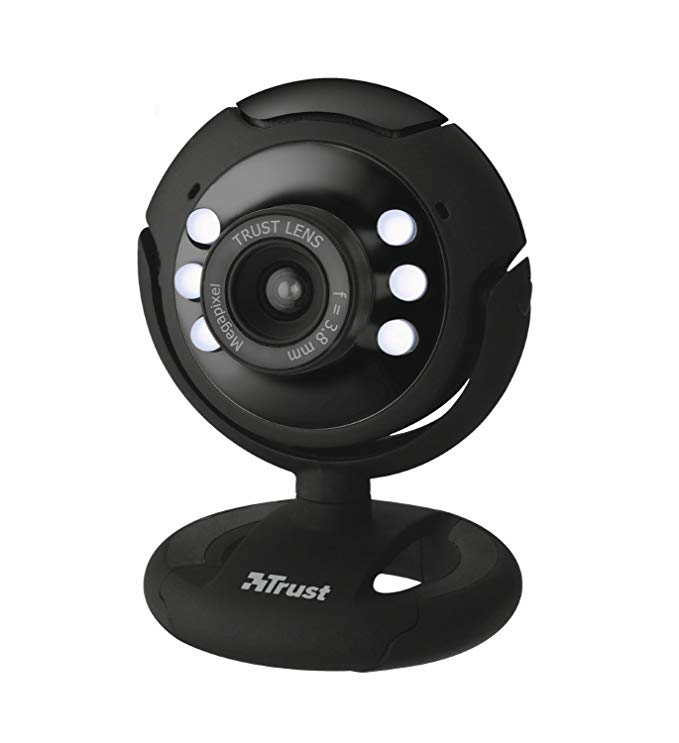
\includegraphics[width=0.25\textwidth]{Immagini/TrustCam.jpg}
	\caption{Camera utilizzata nello stato iniziale del progetto}
	\label{fig:TrustCam}
\end{figure}

È stato però notato che, utilizzando questa camera, non si era in grado di dare sufficienti garanzie di funzionamento stabile in alcune delle più comuni condizioni luminose e ambientali: infatti era alta la variabilità del comportamento della camera al variare delle condizioni luminose, il chè rendeva molto instabile il riconoscimento delle frecce.

Si è deciso quindi di passare ad una camera di tipo industriale, in grado di fornire delle prestazioni più stabili e affidabili.

La scelta è ricaduta sulla camera della casa produttrice \textit{IDS (Imaging Development System)}: si tratta del modello \textit{UI-1221LE-C-HQ} equipaggiata con la lente \textit{BM2420} prodotta dalla \textit{Lensagon} (\href{https://www.lensation.de/product/BM2420/}{lens datasheet}).
\begin{figure}[H]
	\centering
	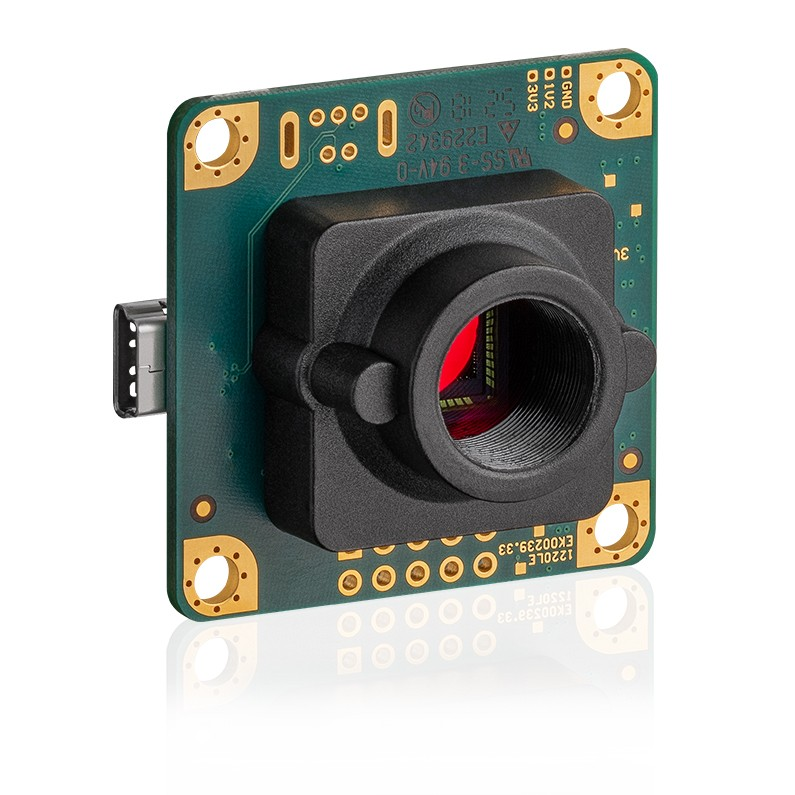
\includegraphics[width=0.3\textwidth]{Immagini/camera-usb2-ueye-le-rev2-boardlevel-m12-1.jpg}
	\caption{Camera utilizzata nello step successivo}
	\label{fig:UeyeCam}
\end{figure}

La camera in Fig.\ref{fig:UeyeCam} ha un'otturatore globale che permette di acquisire tutta l'immagine istantaneamente e non in modo progressivo come la camera  \textit{SpotLight Pro Webcam}.

\section{Come ottenere le immagini dalla camera?}
Per ottenere le immagini dalla camera è stato necessario iscriversi presso il sito web della casa produttrice e scaricare i driver necessari all'installazione e al funzionamento (\href{https://en.ids-imaging.com/manuals-ueye-software.html}{software}).

La videocamera ha diverse opzioni di acquisizione tra cui anche una grandezza dell'immagine diversa dal classico 640x480 pixel ma, per ragioni di semplicità, si è scelto di lasciare invariate le impostazioni di default.

In ogni caso è molto semplice verificare lo stato di funzionamento della camera stessa: è sufficiente, una volta scaricati e installati i software proprietari della casa produttrice, andare ad aprire il software \textit{uEyeDemo} e modificare le impostazioni in base alle proprie necessità.

E' necessario sottolineare come, per essere in grado di ottenere le immagini dalla camera, sia importante assicurarsi che \textit{l'ueye daemon} sia in funzione: esso parte automaticamente dal momento in cui si avvia il PC con la camera già connessa. Nel caso in cui essa venga connessa a caldo è necessario andare ad avviare il \textit{daemon} utilizzando questo comando da terminale, che mette in evidenza come si tratti di un comando per camera usb (nel caso si andasse a lavorare con camera ethernet, servirebbe andare a selezionare la giusta opzione, proposta a terminale):

\begin{quotation}
	\textsl{sudo /etc/init.d/ueyeusbdrc start}
\end{quotation}


\section{CPU consumption}
Un fattore importante nella scelta della camera è l'elevato tempo di utilizzo della CPU da parte della camera \textit{UI-1221LE-C-HQ}. In contrasto, la camera inizialmente scelta vantava un consumo di CPU nettamente inferiore e quindi che più si potrebbe adattare all'installazione su dispositivi mobili e con bassa potenza di calcolo.

\section{Posizionamento camera}

Durante i test e gli esperimenti svolti in laboratorio la videocamera è stata legata ad un palo metallico e fissata con un angolo di inclinazione rispetto ad esso di circa 35 gradi; l'altezza dal pavimento è, inoltre, di circa 83.5 cm


	\chapter{Gestione delle maschere}
	\section{HSV}
Nella strutturazione del progetto ci è venuto molto naturale andare a lavorare con una scala di colori HSV.

Ma perchè non applicare un filtraggio basato su RGB?

Come noto nella letteratura, nell'ambito dell'\textit{image recognition} è usuale il problema di andare a mascherare un colore piuttosto che un altro, come nel nostro caso.

Potremmo voler trovare, sempre per esempio, oggetti di colore rosso, scannerizzando nell'immagine solamente colori (255,0,0) nella scala RGB: con questo approccio andremmo ad applicare una condizione troppo stringente ai colori.
Si potrebbe pensare, come soluzione a questa condizione parecchio stringente, di trovare colori in un range di rossi, come per esempio {(130,0,0);(255,0,0)}: il problema comunque persisterebbe proprio per il fatto che il rosso è ottenuto come combinazione di più colori primari, e non come un solo singolo colore.

Potremmo pensare dunque, di andare a fondo del problema,cambiando gli intervalli dei valori RGB per tutti i colori primari ma sarebbe uno sforzo non secondario e probabilmente con risultati poco significativi.
È necessario un metodo che abbia meno parametri per semplificare l'identificazione dei colori: questo metodo è rappresentato proprio dall'utilizzo del HSV.

\begin{figure}[H]
	\centering
	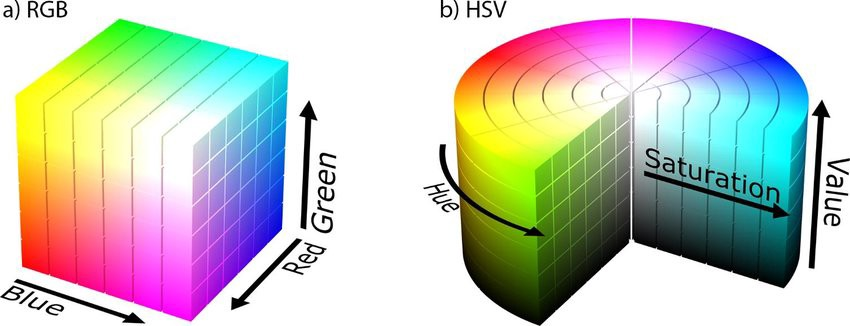
\includegraphics[width=0.5\textwidth]{Immagini/HSV_RGB.jpeg}
	\caption{RGB vs HSV}
	\label{fig:RGB_&_HSV}
\end{figure}

Si può notare come, in Fig \ref{fig:RGB_&_HSV}, il colore rosso sia definito in un range ben chiaro di un solo valore (\textit{Hue}) mentre \textit{Saturation }and \textit{Value} servono solo a limitare ulteriormente la gamma di tonalità di rosso accettabili. 

\section{Frecce o cerchi ?}
Nel progetto utilizzato come punto di partenza, si erano individuati cerchi di diversa grandezza per testare le funzionalità della libreria OpenCV nell'object detection.

Ovviamente l'utilizzo di cerchi limita di molto l'espressività del simbolo in quanto un cerchio non può, per sua natura identificare una direzione, men che meno un verso.
Le frecce sono quindi la soluzione più naturale al problema di identificare con un simbolo una direzione ed un verso che poi, un eventuale robot mobile, potrà seguire.


\section{Maschere}
Le maschere sono fondamentali nel processo di object detection tramite la libreria OpenCV.

Queste ultime sono immagini binarie (bianco e nero) e sono utilizzate da tutte le funzioni di identificazione dei contorni e interpolazione di punti presenti in OpenCV.
La seguente linea di codice permette di identificare tutti gli oggetti di colore rosso e di salvarli nella Matrice \textit{hsv\_red}.

\begin{lstlisting}
	inRange(original_image_hsv, Scalar(MinH_R, MinS_R, MinV_R), Scalar(MaxH_R, MaxS_R, MaxV_R), hsv_red);
\end{lstlisting}



\section{Erosione e dilatazione}
L'erosione e la dilatazione sono tecniche note allo stato dell'arte attuale utili per rimuovere rumore da una immagine.

\begin{figure}[H]
	\centering
	
\includegraphics[width=0.5\textwidth]{Immagini/erosion_dil.png}
	\caption{Erosione e dilatazione}
	\label{fig:erosion_dil}
\end{figure}

Nel caso preso in considerazione da questo report è stato necessario applicare la tecnica di erosione solamente alla parte inferiore dell'immagine in quanto, se applicata nella parte superiore, avrebbe eliminato oltre al rumore anche un'eventuale freccia che sarebbe apparsa molto piccola.

Da sottolineare è il fatto che la tecnica di erosione e successiva dilatazione è stata applicata solamente alle figure rettangolari rosse in quanto la funzione di dilatazione prevede un kernel per la computazione del filtro: dato un kernel definito da una x e una y risulterebbe quanto mai complesso effettuare una dilatazione che rassomigli poi ad una forma triangolare.
	\chapter{Identificazione delle forme}
	\section{Definizione del problema}
Il capitolo precedente ha mostrato come sia possibile ottenere dei contorni, delle figure data un' immagine a colori.
È ora necessario identificare la forma di ciascuno di questi contorni riconoscendo così i vari quadrati e rettangoli presenti nell'immagine che avessero, una volta acquisiti dalla camera, il colore specificato. Come ultimo passaggio va svolto il controllo per verificare che esista o meno una freccia; quest'ultima altro non è che un triangolo e un rettangolo sufficientemente vicini fra di loro.

\section{Interpolazione}
Per approssimare il contorno ottenuto e filtrato attraverso le mask, come spiegato nel Capitolo 3, è necessario usare una funzione che approssima il contorno individuato con un altro poligono avente meno vertici così che la distanza tra di essi sia inferiore ad una certa soglia. Tale funzione è così definita nella libreria OpenCV:

\begin{quotation}
	\textsl{void approxPolyDP(InputArray curve, OutputArray approxCurve, double epsilon, bool closed)}
\end{quotation}

Si è reso necessario effettuare un tuning del parametro \textsl{double epsilon} in quanto, per frecce diverse, a distanza variabile e con orientazione non fissa sono stati individuati differenti valori ottimali. Il valore che più si adattava a tutti i casi presi in considerazione è stato ottenuto sperimentalmente e corrisponde a \textsl{double epsilon=0.045}.

La funzione di cui sopra restituisce quindi una lista di poligoni ognuno dei quali è descritto da una lista di vertici.
Il passo successivo è stato cercare nella lista dei poligoni un elemento che avesse 4 lati nel caso di un rettangolo e 3 in quello di un triangolo:

\begin{lstlisting}
	if(result->total >= 3  && result->total <= 3 && fabs(cvContourArea(result, CV_WHOLE_SEQ))>lower_area_triang)
\end{lstlisting}
\begin{lstlisting}
	if(result->total >= 4  && result->total <= 6 && fabs(cvContourArea(result, CV_WHOLE_SEQ))>lower_area_rect)
\end{lstlisting}

Sempre per via sperimentale è stato possibile scoprire che vincolando il poligono che approssima il quadrilatero cercato ad avere tra i 4 e i 6 lati, la probabilità di riconoscere correttamente un rettangolo aumentava.Per il triangolo questo non si è reso necessario vista la buona probabilità di successo nella ricerca vincolata a 3 lati.

Ottenuti ora tutti i triangoli e i rettangoli sufficientemente grandi nella figura va affrontato il problema del riconoscimento di ogni freccia presente nel seguente modo:
\begin{itemize}
	\item \textbf{} per ciascun rettangolo identificato, si calcola la distanza che intercorre tra esso e ogni triangolo riconosciuto. Per calcolare la distanza tra due figure è necessario:
	\begin{itemize}
		\item \textbf{}definire il centro del rettangolo, tramite funzioni della libreria OpenCV
		\item \textbf{}ottenere il baricentro del triangolo
		\item \textbf{}calcolare la distanza cartesiana tra i due punti appena individuati
	\end{itemize}
	\item \textbf{} si tiene in considerazione solamente la distanza minore calcolata.
	\item \textbf{} si confronta suddetto valore con una soglia sperimentale; se questo valore è minore allora si può assumere che il triangolo e il quadrato presi in considerazione siano una freccia, altrimenti si scarta la coppia.
	\item \textbf{} la freccia appena rilevata viene aggiunta alla lista delle frecce rilevate nell'immagine.
\end{itemize}
Per ogni freccia, che ora altro non è che una coppia di punti,
\begin{equation}
	\begin{split}
		C_{triangolo}=(x_t,y_t)\\ 
		C_{rettangolo}=(x_r,y_r)
	\end{split}
\end{equation}

vanno identificati nell'ordine:
\begin{itemize}
	\item \textbf{}il centro della freccia, ottenuto come il punto medio del segmento che collega i due centri che definivano la freccia precedentemente.
	$$
		C_{freccia}=(\dfrac{x_t+x_r}{2},\dfrac{y_t+y_r}{2})
	$$
	\item \textbf{}L'inclinazione della freccia nel piano, calcolata come:
		\begin{equation}
			\begin{split}
				\phi=atan(\frac{\Delta y}{\Delta x}), dove\\
				\Delta y=y_t-y_r\\
				\Delta x=x_t-x_r
			\end{split}
		\end{equation}
	\item \textbf{}L'area dell'oggetto freccia, ricavata come somma dell'area del triangolo e del quadrato.
	
	
	

\end{itemize}	
	\chapter{Dalle pixel coordinates alle world coordinates}
	\section{Definizione del problema}
Nel capitolo precedente è stato illustrato un metodo atto all'identificazione delle frecce che rientrano nel campo visivo della camera.
Viene ora trattato come sia possibile ottenere la posizione della freccia, precedentemente identificata, nelle coordinate 3D (U,V,W) rispetto alla base del robot.

\begin{figure}[H]
	\centering
	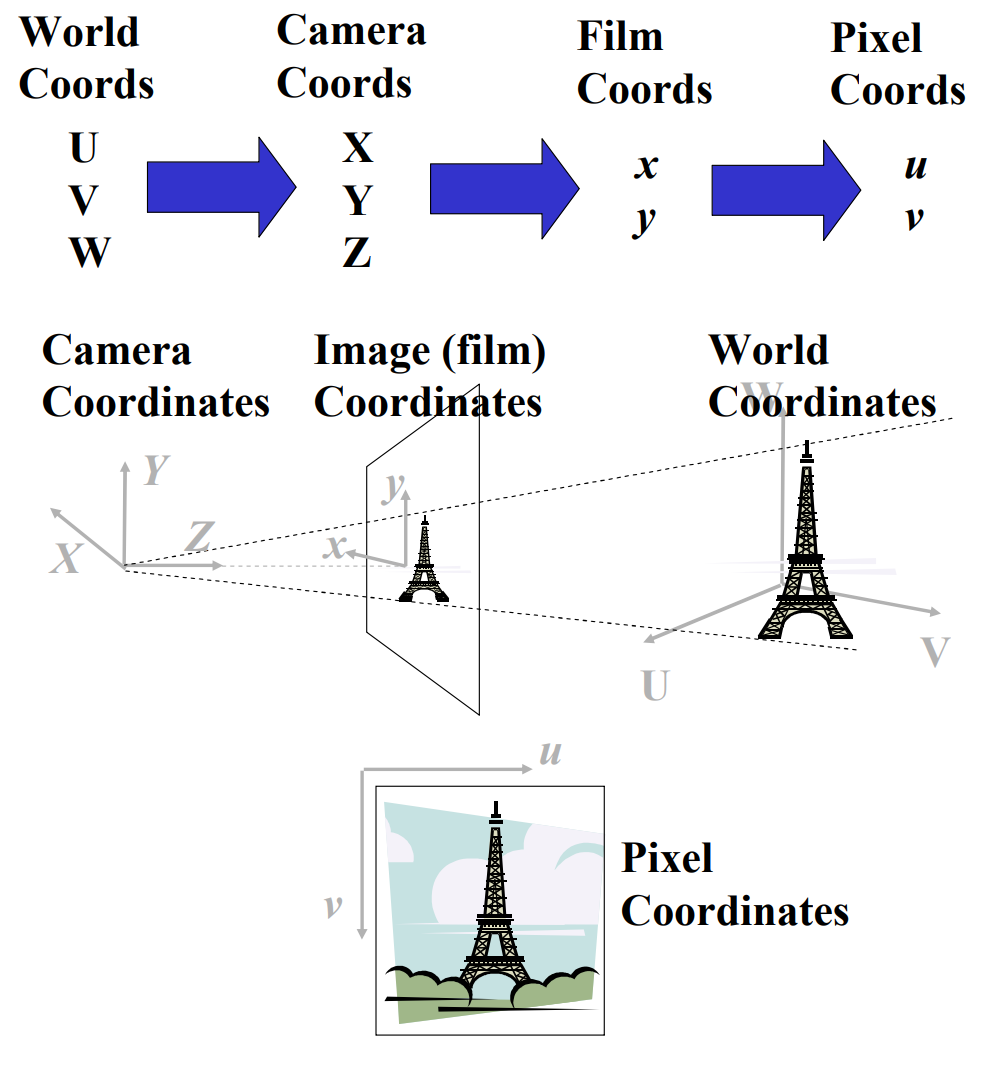
\includegraphics[width=0.8\textwidth]{Immagini/world_coords.png}
	\caption{Schema concettuale delle diverse coordinate in gioco}
	\label{fig:fromcamtoworld}
\end{figure}

Come si vede in figura \ref{fig:fromcamtoworld}, sono necessarie tre trasformazioni per ottenere, a partire dalle \textit{world coordinates}, le \textit{pixel coordinates}.

Nel caso specifico del sistema preso in considerazione all'interno di questo report, il problema risulta essere l'opposto: dalle coordinate nella camera è necessario ottenere la posizione globale dell'oggetto effettuando una trasformazione inversa.

Si analizzeranno ora le singole trasformazioni che permetteranno alla fine di ottenere il risultato voluto.

\section{Da \textit{world coordinates} a \textit{camera coordinates}}
\begin{figure}[H]
	\centering
	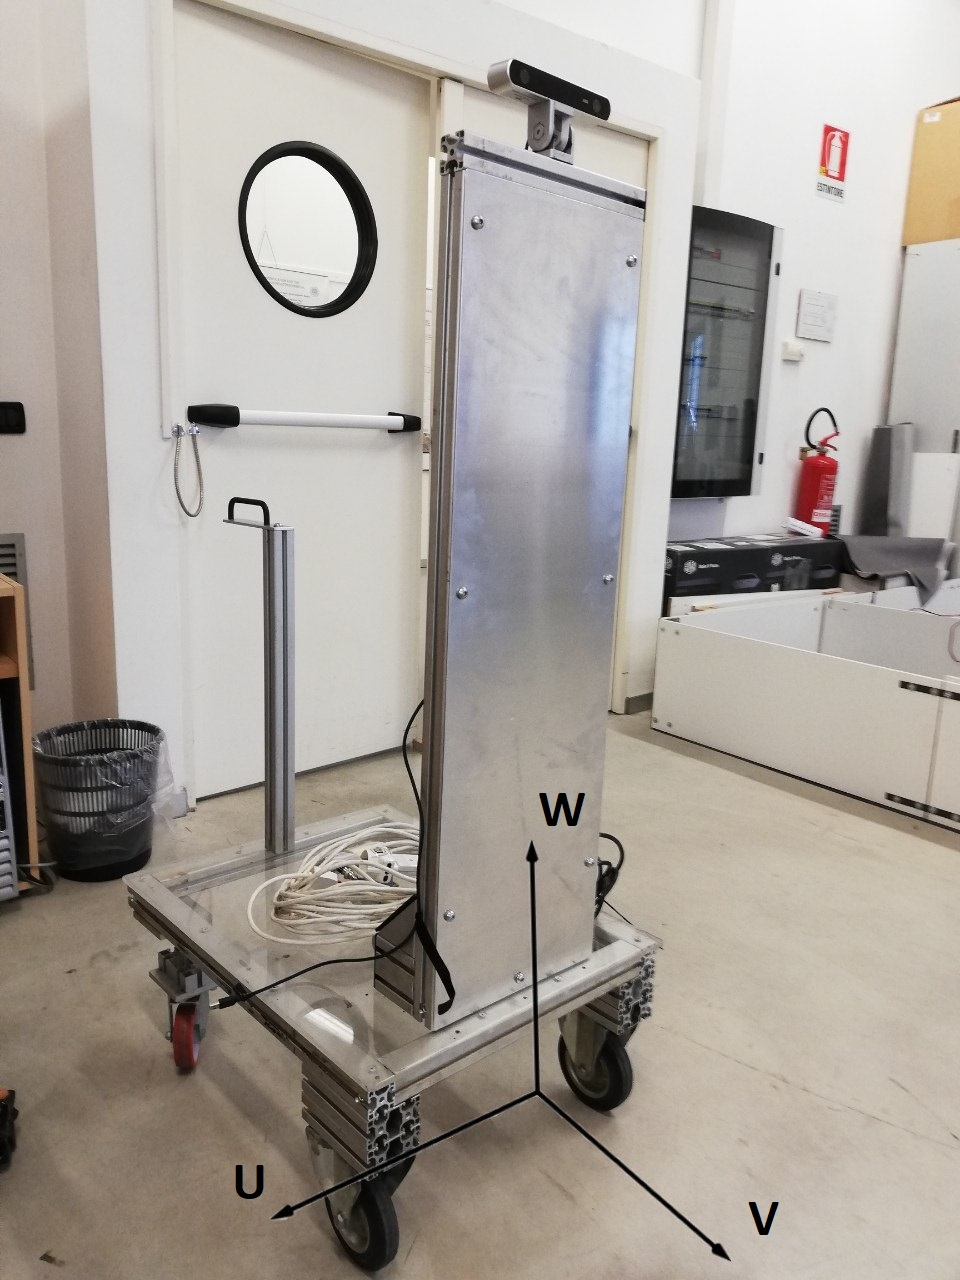
\includegraphics[width=0.4\textwidth]{Immagini/SupportoCamera_asse1.jpg}
	\caption{Posizione del world frame}
	\label{fig:worldframe}
\end{figure}

Partendo da un sistema di riferimento solidale al robot e posto all'altezza del pavimento, che identifichiamo come sistema globale, è possibile definire una matrice di rototraslazione per ottenere il sistema di riferimento solidale al centro della camera.

\begin{equation*}
R_{worldcam} = R_{traslazione} \cdot R_{rotazione} =\\
\begin{pmatrix}
1 & 0 & 0 & 0 \\
0 & 1 & 0 & 0 \\
0 & 0 & 1 & h_{cam} \\
0 & 0 & 0 & 1 \\
\end{pmatrix} \cdot
\begin{pmatrix}
1 & 0 & 0 & 0 \\
0 & cos(\dfrac{\pi}{2} + cam\_incl) & -sin(\dfrac{\pi}{2} + cam\_incl) & 0 \\
0 & sin(cam\_incl + \dfrac{\pi}{2}) & cos(cam\_incl + \dfrac{\pi}{2}) & 0 \\
0 & 0 & 0 & 1 \\
\end{pmatrix}
\end{equation*}
\footnote{\textit{cam incl} corrisposnde, all'interno del codice, alla variabile \textit{cam inclination}}

È stata effettuata una traslazione lungo l'asse W in quanto la camera è posta esattamente sopra l'origine del sistema $O_{UVW}$ ed una rotazione rispetto all'asse U di $ \dfrac{\pi}{2}$ in quanto, per convenzione, si associa all'asse delle Z la profondità nel frame solidale alla camera.

A questo punto è necessario effettuare un'altra rotazione di \textit{cam inclination} gradi rispetto all'asse X a seconda dell'inclinazione alla quale si sceglie di far lavorare la camera, come si vede in figura ~\ref{fig:cameraSupport}.

\begin{figure}
	\centering
	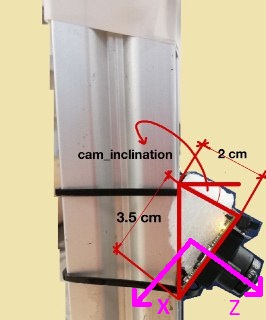
\includegraphics[width=0.5\textwidth]{Immagini/CameraSupport_2.jpg}
	\caption{Posizionamento della camera su supporto metallico}
	\label{fig:cameraSupport}
\end{figure}

\section{Da \textit{camera coordinates} a \textit{film coordinates}}
\begin{figure}[H]
	\centering
	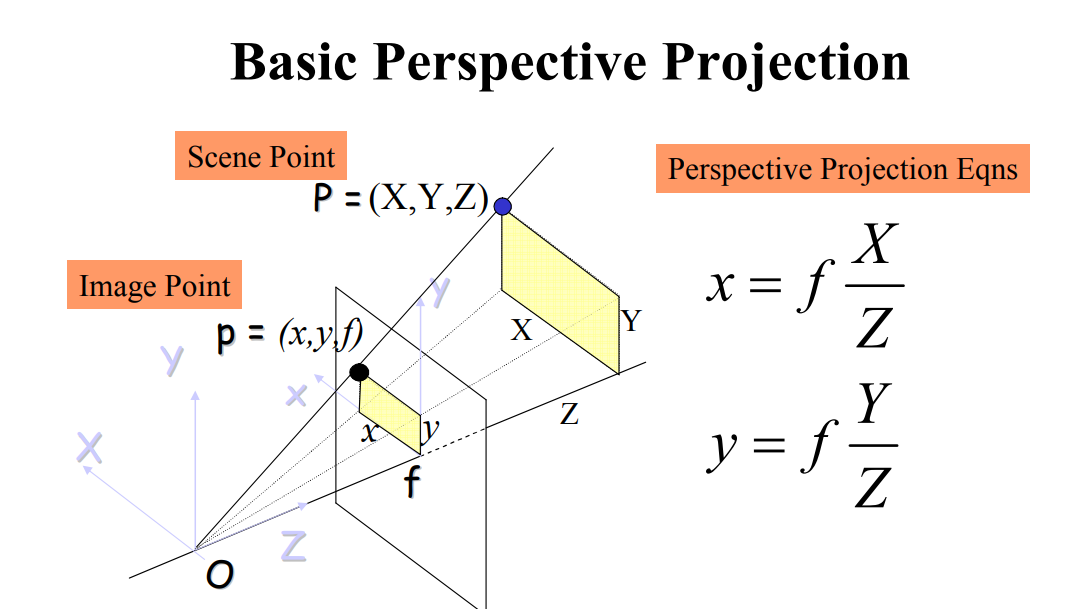
\includegraphics[width=0.7\textwidth]{Immagini/perspective_projection.png}
	\caption{Descrizione del problema}
	\label{fig:perspective_projection}
\end{figure}
Nello schema in figura \ref{fig:perspective_projection}, \textit{f} rappresenta il fuoco della camera: si tratta di un parametro ottenibile attraverso la procedura di calibrazione, il quale può, come il centro della camera, essere scomposto in due componenti $f_x$ e $f_y$, utilizzati rispettivamente, per trasformazioni lungo l'asse $x$ e lungo l'asse $y$.

\section{Da \textit{film coordinates} a \textit{pixel coordinates}}

\begin{figure}[H]
	\centering
	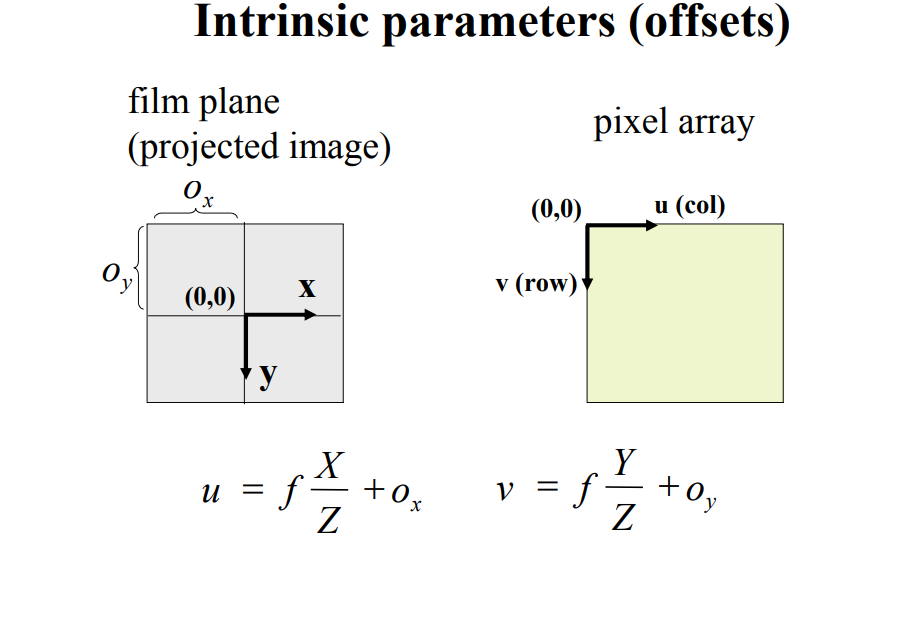
\includegraphics[width=0.7\textwidth]{Immagini/intrinsic_parameters.png}
	\caption{Descrizione dell'ultima trasformazione}
	\label{fig:intrinsic_parameters}
\end{figure}
In figura \ref{fig:intrinsic_parameters}, i termini $ O_{x}$ e $ O_{y} $ rappresentano i centri della camera e sono anch'essi ricavabili tramite la procedura di calibrazione della camera.

\section{Problema inverso}
\begin{figure}[H]
	\centering
	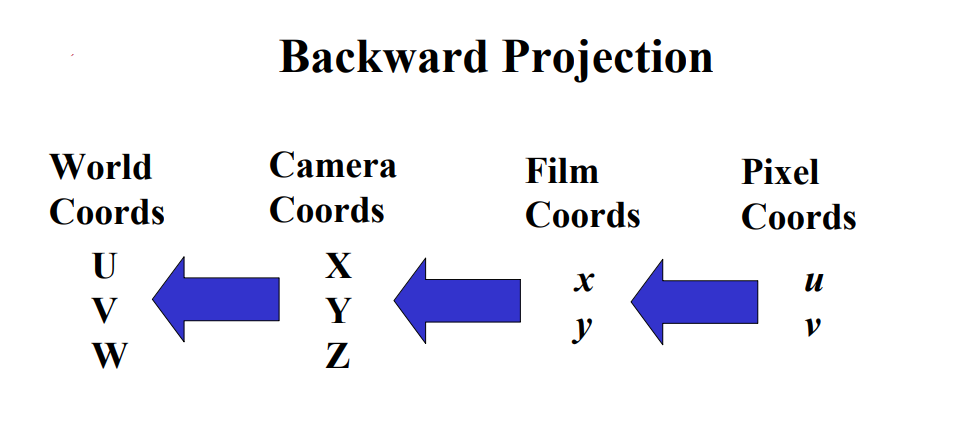
\includegraphics[width=0.7\textwidth]{Immagini/backward.png}
	\caption{Problema inverso}
	\label{fig:backward}
\end{figure}

Come si vede in figura \ref{fig:backward}, si deve ora affrontare il processo inverso siccome, nel nostro caso, si hanno a disposizione \textit{u} e \textit{v} e si vogliono ottenere \textit{U,V,W}.

Come già detto in precedenza, $ O_{x}$ e $ O_{y} $ e \textit{f} sono ottenibili tramite calibrazione. e quindi:

\begin{equation}
\begin{split}
x = u -O_{x}\\
y = v -O_{y}
\end{split}
\end{equation}

In questo modo sono quindi state ottenute le equazione del film coordinates. 

È ora necessario ottenere le camera coordinates. Per fare ciò è necessario conoscere il valore di Z (ovvero la profondità), la quale è ottenibile in due modi:
\begin{itemize}
	\item utilizzando una camera con sensore di profondità
	\item assumendo che gli oggetti inquadrati dalla camera siano sempre posti su un piano di cui si conosce l'equazione.
\end{itemize}
La seconda assunzione è, nella realtà dei fatti, un'ipotesi corretta e applicabile in quanto, nel nostro caso, gli oggetti e le frecce giaceranno sempre sul pavimento.

È quindi richiesto di calcolare l'equazione del pavimento nel camera frame:
\begin{itemize}
	\item $z = 0$ rappresenta l'equazione del piano se fosse nel world frame
	\item $z \cdot R_{worldcam} = 0$ indica il piano così calcolato è la descrizione dal punto di vista matematico del pavimento dal punto di vista della camera
	\begin{figure}[H]
		\centering
		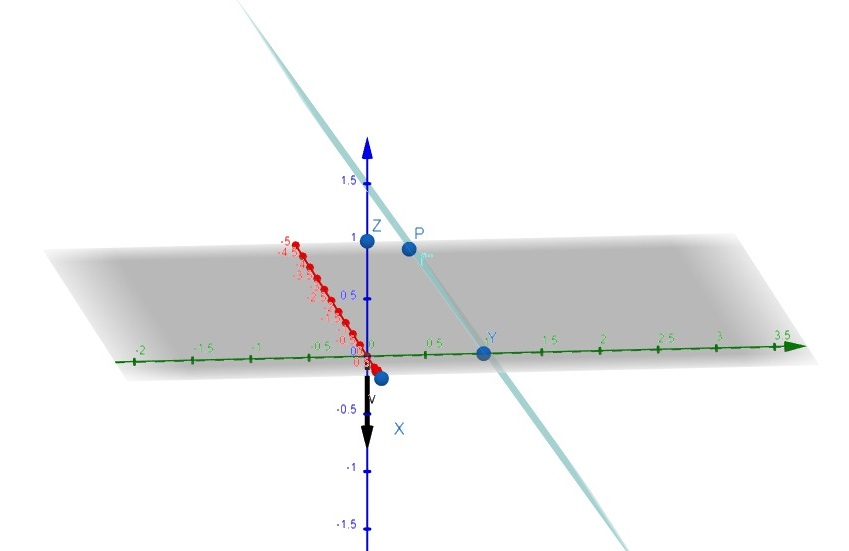
\includegraphics[width=0.7\textwidth]{Immagini/piano_camera.jpeg}
		\caption{Piano del pavimento nel camera frame}
		\label{fig:piano_camera}
	\end{figure}
	\item si può calcolare il fattore di scala s dato un generico piano $ax+by+cz+d=0$
		\begin{equation}
		\begin{split}
		s = \dfrac{-d}{aX'+bY'+c}	
		\end{split}
		\end{equation}
	dove
		\begin{equation}
		\begin{split}
		X'=\dfrac{x}{f_x}=\dfrac{X}{Z}\\
		Y'=\dfrac{y}{f_y}=\dfrac{Y}{Z} \\
		\end{split}
		\end{equation}
	che sono le coordinate normalizzate rispetto a Z.
	\item Dunque, come ultimo passaggio si moltiplica tutto per il fattore di scala:
		\begin{equation}ù
		\begin{split}
		X=X' \cdot s\\
		Y=Y' \cdot s\\
		Z=S
		\end{split}
		\end{equation}
\end{itemize}

Per ottenere le equazione nel world frame si deve dunque utilizzare la matrice inversa:

$$
\begin{pmatrix}
U  \\
V  \\
W  \\
1  \\
\end{pmatrix}
=R_{worldcam}^{-1}\cdot
\begin{pmatrix}
X  \\
Y  \\
Z  \\
1  \\
\end{pmatrix}
$$

	\begin{thebibliography}{9}
		\bibitem{bib1}
		\emph{Descrizione della camera}
		\url{https://en.ids-imaging.com/store/ui-1221le-rev-2.html}
		
		\bibitem{bib2}
		\emph{Manuale della camera}
		\url{https://en.ids-imaging.com/IDS/datasheet_pdf.php?sku=AB02422}
		
		\bibitem{bib3}
		\emph{Manuale della lente}
		\url{https://www.lensation.de/product/BM2420/}
		
		\bibitem{bib4}
		\emph{Ueye cam e ROS}
		\url{http://wiki.ros.org/ueye}
		
		\bibitem{bib5}
		\emph{HSV vs RGB}
		\url{https://medium.com/neurosapiens/segmentation-and-classification-with-hsv-8f2406c62b39}
		
		\bibitem{bib6}
		\emph{HSV vs RGB}
		\url{https://handmap.github.io/hsv-vs-rgb/}
		%%%%%%%%%%%%%%%%%%%%%%%%%%%%%%%%%%%%%%%%%%%%
		\bibitem{bib7}
		\emph{Camera Projection I}
		\url{http://www.cse.psu.edu/~rtc12/CSE486/lecture12.pdf}
		%%%%%%%%non so dove metterle%%%%%%%%%%%%%%%%%%%
		\bibitem{bib8}
		\emph{Camera Projection II}
		\url{http://www.cse.psu.edu/~rtc12/CSE486/lecture13.pdf}
		
		\bibitem{bib9}
		\emph{Coordinate omogenee}
		\url{http://robotics.unibg.it/teaching/robotics/pdf/14_Geometria3D.pdf}
		%%%%%%%%%%%%%%%%%%%%%%%%%%%%%%%%%%%%%%%%%%%%%%%%
		\end{thebibliography}

\end{document}
